\chapter{Results} \label{ch:results}
The angular power spectra derived in \autoref{ch:methodology} represent theoretical predictions 
for a specific set of model parameters. To assess how well these parameters could be recovered 
from an actual measurement, the likelihood is assumed to be Gaussian around the fiducial model. 
Under this assumption, the expected parameter covariance follows directly from the Fisher 
information matrix. Since the true posterior may be broader and non-Gaussian, the uncertainties 
quoted here should be regarded as optimistic estimates of the achievable constraints.

\section{Fisher Matrix} \label{sec:fisher_matrix}
The Fisher matrix quantifies how sensitively the observables respond to variations in the model
parameters and therefore how much information a given measurement carries about them. For a set
of tracer fields whose harmonic coefficients are Gaussian distributed, the Fisher matrix of the
angular power spectra $C_\ell$ is given by~\cite{Tegmark_1997, Reischke_2021}
\begin{equation}\label{eq:fisher}
    F_{ij}
    =
    f_{\mathrm{sky}}
    \sum_{\ell=\ell_{\mathrm{min}}}^{\ell_{\mathrm{max}}}
    \frac{2\ell+1}{2}\,
    \operatorname{Tr}
    \left[
        C_{\ell}^{-1}\,
        \frac{\partial C_{\ell}}{\partial \theta_i}\,
        C_{\ell}^{-1}\,
        \frac{\partial C_{\ell}}{\partial \theta_j}
    \right],
\end{equation}

where $\theta_i$ denotes the $i$-th model parameter, $C_\ell$ is the matrix of auto- and
cross-power spectra over all tracer pairs, the trace runs over the tracer indices, and
$f_{\mathrm{sky}}$ accounts for the fact that only a fraction of the celestial sphere is observed.

The derivatives entering \autoref{eq:fisher} are evaluated by central finite differencing,

\begin{equation}\label{eq:finite_difference}
    \frac{\partial C_{\ell}}{\partial \theta_i}
    =
    \frac{C_{\ell}(\theta_i + h_i) - C_{\ell}(\theta_i - h_i)}{2 h_i},
\end{equation}

with step sizes $h_i = 0.01\,\theta_i$. The two parameters considered here are the amplitude
$b_0$ and the evolution exponent $\delta$ of the FRB host bias of \autoref{eq:frb_bias}; all
cosmological parameters are held fixed at the values listed in \autoref{tab:fiducial_cosmology}.
The fiducial values and corresponding step sizes are summarized in \autoref{tab:fisher_setup}.

\begin{table}[H]
    \centering
    \caption{Fiducial values of the FRB bias parameters of \autoref{eq:frb_bias} and the
    corresponding displacements used in the central finite difference of
    \autoref{eq:finite_difference}. The step size is one percent of the respective fiducial value.}
    \label{tab:fisher_setup}
    \begin{tabular}{llSSS}
        \toprule
        Progenitor class & Parameter & {Fiducial $\theta_i$} & {$\theta_i + h_i$} & {$\theta_i - h_i$} \\
        \midrule
        Magnetars     & $b_0$      & 1.0 & 1.010 & 0.990 \\
        Magnetars     & $\delta$   & 0.8 & 0.808 & 0.792 \\
        Neutron stars & $b_0$      & 1.5 & 1.515 & 1.485 \\
        Neutron stars & $\delta$   & 0.2 & 0.202 & 0.198 \\
        \bottomrule
    \end{tabular}
\end{table}

The sum in \autoref{eq:fisher} is carried out over the multipole range $\ell \in [10,\,1000]$
introduced in \autoref{sec:fiducial_cosmology}. The FRB-only forecast adopts the full FRB
footprint of $f_{\mathrm{sky}} = 0.9$ given in \autoref{tab:frb_surveys}, whereas the joint
forecast is restricted to the overlap with the KiDS field, $f_{\mathrm{sky}} = 0.0327$,
corresponding to the $\qty{1347}{\deg\squared}$ quoted in
\autoref{sec:galaxy_redshift_distribution}.

Inverting the Fisher matrix yields the parameter covariance $\mathrm{Cov} = F^{-1}$, whose
diagonal entries define the marginalized errors $\sigma_i = \sqrt{\mathrm{Cov}_{ii}}$~\cite{Coe_2009}.
To compress the two-dimensional constraint into a single number, the figure of merit

\begin{equation}\label{eq:fom}
    \mathrm{FoM} = \frac{1}{\sqrt{\det \mathrm{Cov}}}
\end{equation}

is used, which is inversely proportional to the area of the confidence ellipse, so that larger
values correspond to tighter constraints~\cite{Wang_2008}.

\section{Forecast Constraints} \label{sec:forecast_constraints}
The forecast is evaluated for all four combinations of the two progenitor classes of
\autoref{tab:frb_bias} and the two FRB survey configurations of \autoref{tab:frb_surveys}. The
resulting confidence ellipses are shown in \autoref{fig:fisher_comparison}, and the marginalized
errors together with the figures of merit are listed in \autoref{tab:fisher_constraints}.

\begin{figure}[H]
    \centering
    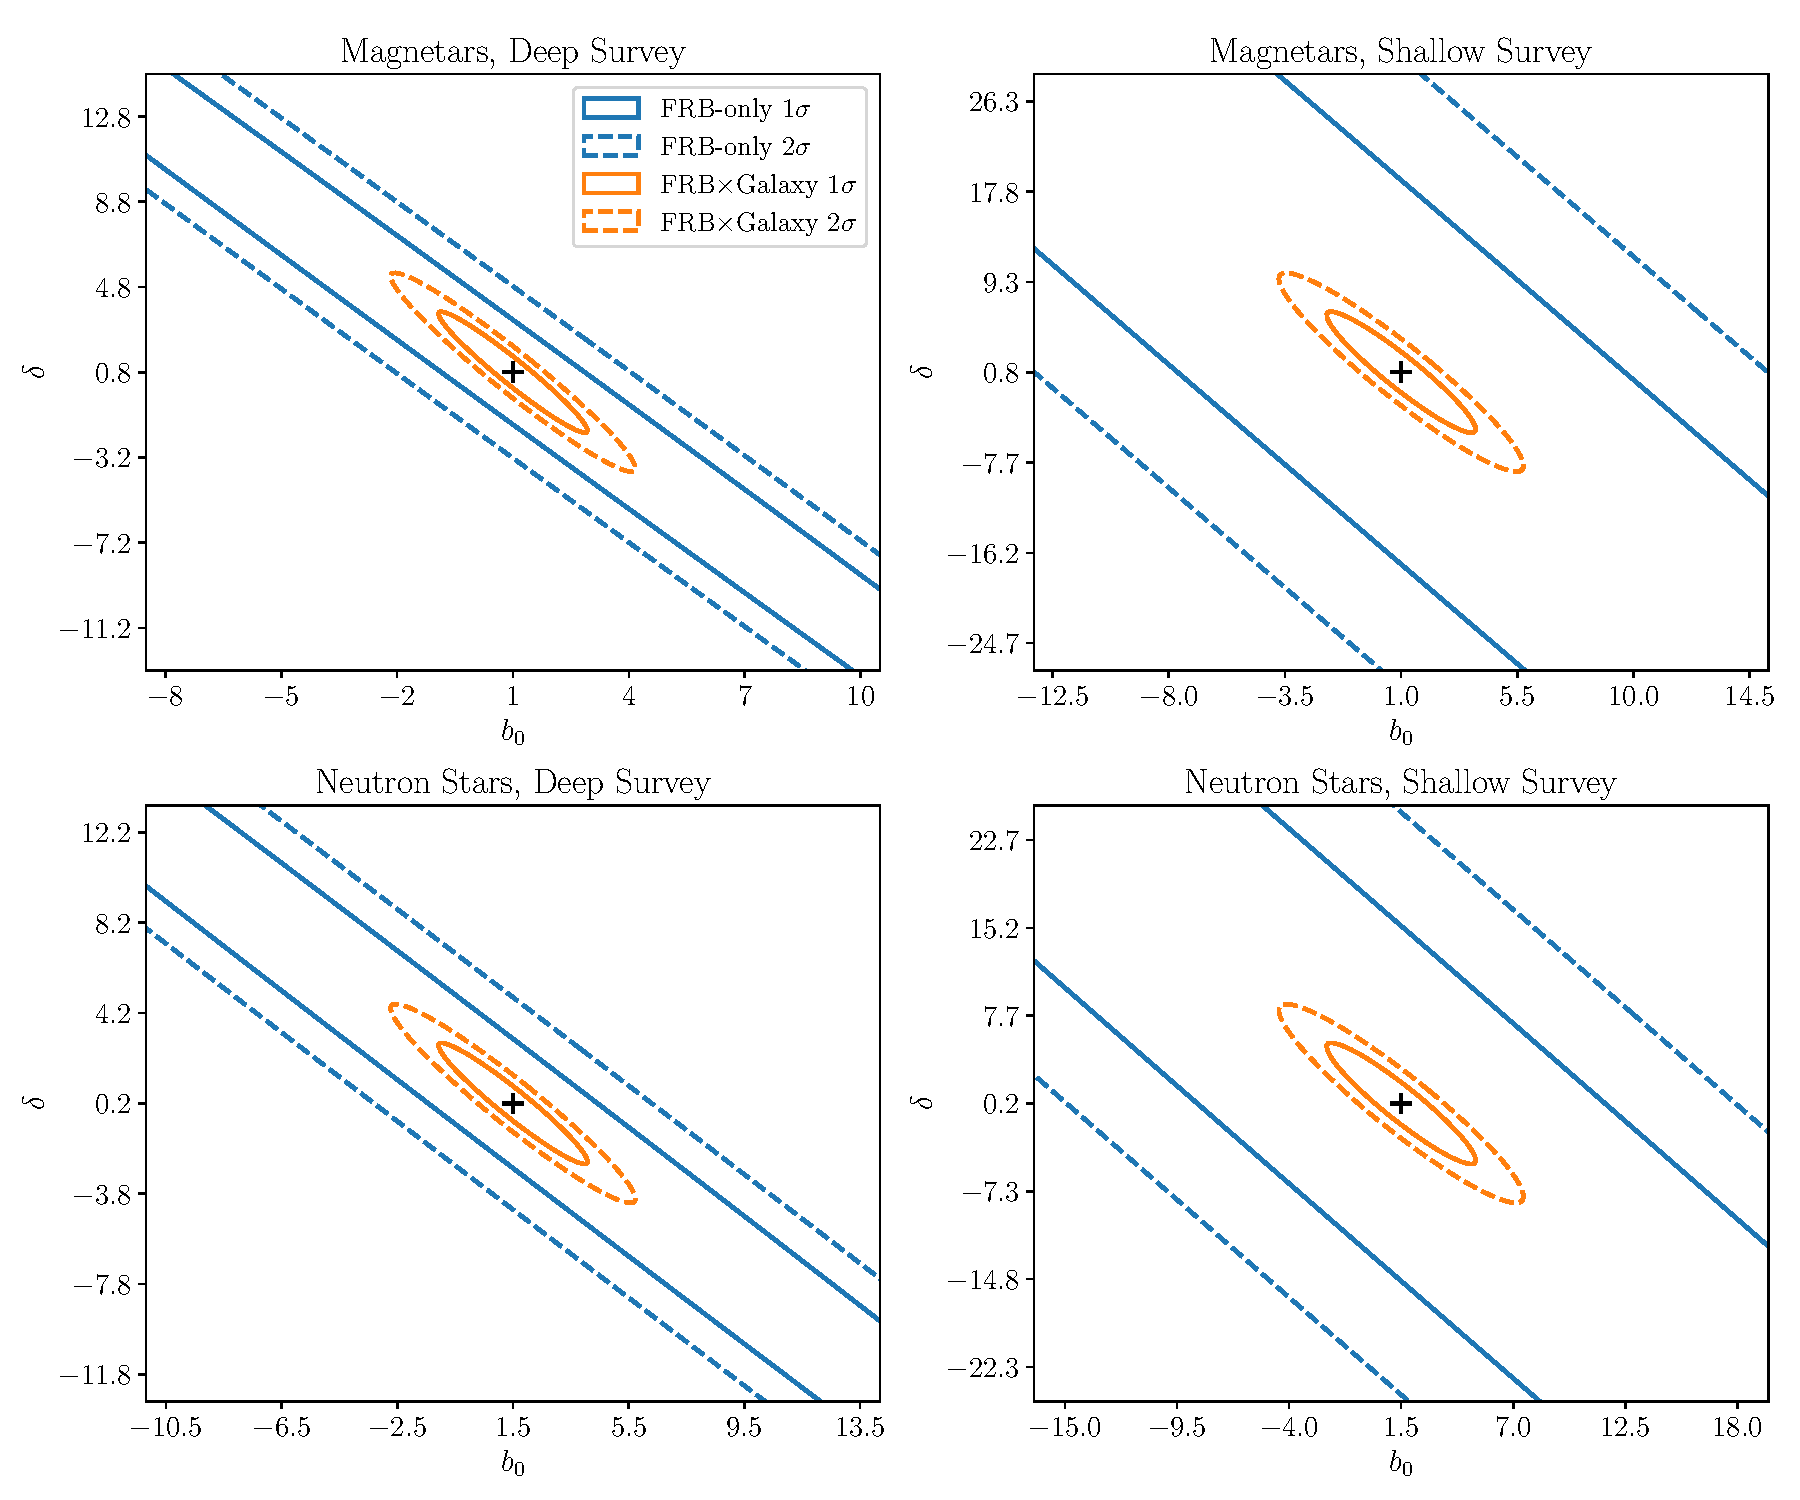
\includegraphics[width=\textwidth]{../programming/frb-cosmology/plots/fisher/fisher_comparison_2x2.pdf}
    \caption{Fisher forecast in the $b_0\,$--$\,\delta$ plane for the two progenitor classes and the two
    FRB survey configurations. Shown are the $1\sigma$ and $2\sigma$ contours obtained from the FRB
    auto-correlation alone in blue and from the joint analysis of the FRB sample with the six tomographic
    KiDS bins in orange. The black cross marks the fiducial parameter values. The FRB-only contours extend far
    beyond the plotted range in every panel.}
    \label{fig:fisher_comparison}
\end{figure}

\begin{table}[H]
    \centering
    \small
    \setlength{\tabcolsep}{0.5pt}
    \caption{Marginalized $1\sigma$ errors on the FRB bias parameters and the corresponding
    figure of merit of \autoref{eq:fom}, obtained from the FRB auto-correlation alone
    and from the joint analysis with the six KiDS-Legacy tomographic bins.
    The last column gives the gain in the figure of merit,
    $\mathrm{FoM}^{\mathrm{FRB}\times\mathrm{gal}}/\mathrm{FoM}^{\mathrm{FRB}}$.}
    \label{tab:fisher_constraints}
    \begin{tabular}{llSSSSSSS}
        \toprule
        & &
        \multicolumn{2}{c}{$\sigma_{b_0}$} &
        \multicolumn{2}{c}{$\sigma_{\delta}$} &
        \multicolumn{3}{c}{FoM} \\
        \cmidrule(lr){3-4}
        \cmidrule(lr){5-6}
        \cmidrule(lr){7-9}

        Progenitor & Configuration
        & {FRB} & {FRB$\times$gal}
        & {FRB} & {FRB$\times$gal}
        & {FRB} & {FRB$\times$gal} & {Gain} \\

        \midrule

        Magnetars     & Deep
        & 23.48 & 1.27
        & 31.07 & 1.88
        & 0.0263 & 1.59 & 60.7 \\

        Magnetars     & Shallow
        & 91.32 & 1.91
        & 190.60 & 3.76
        & 0.0009 & 0.41 & 448.7 \\

        Neutron stars & Deep
        & 33.04 & 1.70
        & 32.35 & 1.77
        & 0.0160 & 1.15 & 72.1 \\

        Neutron stars & Shallow
        & 101.0 & 2.42
        & 153.00 & 3.41
        & 0.0010 & 0.34 & 348.3 \\

        \bottomrule
    \end{tabular}
\end{table}

The FRB auto-correlation alone does not constrain the host bias: marginalized errors range from
$\sigma_{b_0} = 23.5$ to $101$, exceeding the fiducial values by one to two orders of magnitude.
Adding the galaxy sample reduces these to $\sigma_{b_0} = 1.27$--$2.42$ and
$\sigma_{\delta} = 1.77$--$3.76$, an improvement by factors of $17$--$51$ in the individual
parameters and $61$--$449$ in the figure of merit. The joint analysis is therefore not a marginal
refinement but the reason a measurement becomes feasible in the first place.

\section{Discussion} \label{sec:results_discussion}

As shown in \autoref{fig:frb_cell_shotnoise}, the FRB shot noise exceeds the clustering signal
by two to three orders of magnitude at every multipole, rendering the auto-spectrum essentially
uninformative. The cross-correlation with the much denser KiDS galaxy field circumvents this
because the cross-spectrum carries no FRB shot-noise contribution, as discussed in
\autoref{sec:cross_correlation_analysis}.

%\pagebreak
%The orientation of the contours in \autoref{fig:fisher_comparison} is equally informative. In all
%four panels, the parameters are anti-correlated because the FRB auto-spectrum integrates over the
%full FRB redshift kernel but is locally most sensitive to a weighted effective redshift. Thus, an
%increase in $b_0$ can be compensated by a decrease in $\delta$, leaving the combination
%$b_0(1+z_{\mathrm{eff}})^\delta$ approximately unchanged. The FRB-only contours are therefore highly
%elongated and constrain essentially one parameter combination. The joint contours are smaller and
%visibly rounder. This is a genuinely tomographic effect: the six galaxy bins weight the FRB kernel
%over different redshift ranges, as indicated by the bin dependence of the cross-spectra in
%\autoref{fig:cross_survey}. The bias is consequently probed with several different effective
%redshift weightings, breaking the degeneracy through redshift leverage rather than increased
%signal-to-noise alone.
%\pagebreak

Comparing the two survey configurations, the deep sample outperforms the shallow one in every
case, as expected from its ten-fold larger burst count and correspondingly lower shot noise.
However, this advantage propagates differently into the two forecasts: in the FRB-only case the
deep configuration improves $\sigma_{b_0}$ by a factor of three to four, while in the joint case
the gain is only about $1.4$--$1.5$. Once the constraint is no longer dominated by FRB shot noise,
increasing the burst count becomes considerably less effective, and the radial overlap between the
FRB and galaxy samples takes over as the limiting factor.

VIELLEICHT GAR NICHT NOETIG DIESER PART HIER

A comparison of the two progenitor classes requires some care, as their fiducial values differ.
In absolute terms the magnetar model yields smaller errors, but relative to the respective fiducial
amplitudes both models are constrained equally well, with $\sigma_{b_0}/b_0 = 1.13$ and $1.27$
for the deep configuration. The more consequential question is whether the two models can be
distinguished: the fiducial separation of $\Delta b_0 = 0.5$ and $\Delta \delta = 0.6$ lies
comfortably within the $1\sigma$ contours of the joint forecast, so the cross-correlation with
KiDS improves the measurement by more than two orders of magnitude in the figure of merit but
does not yet reach the precision required to discriminate between a prompt magnetar and a delayed
neutron-star origin. This is not a statement about the method but about sky area: the Fisher
information of \autoref{eq:fisher} scales linearly with $f_{\mathrm{sky}}$, and the natural path
to improvement is a wider galaxy survey, which is taken up in \autoref{sec:outlook}.